
\section{Parte 2: Análisis dinámico del pozo finito asimétrico [50 puntos]}
 
Consideremos ahora el pozo finito asimétrico definido por el potencial
\begin{equation}
U(x) = \begin{cases} U_1, & x < 0, \\ 0, & 0 \leq x < L, \\ U_2, & x \geq L, \end{cases} \qquad \{U_1, U_2\} > 0, \qquad U_2 \geq U_1, \qquad c \equiv \frac{U_2}{U_1} \geq 1, \tag{10}
\end{equation}

\begin{figure}
    \centering
    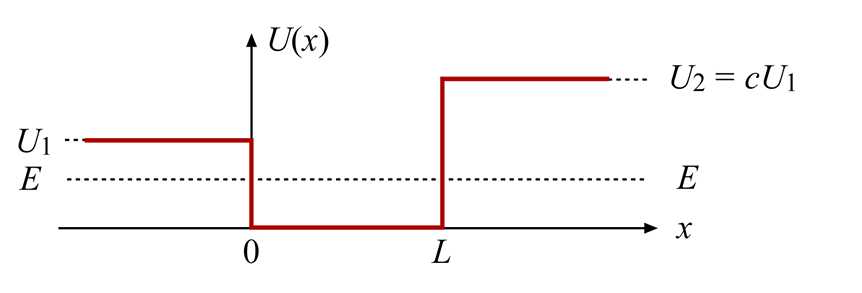
\includegraphics[width=0.5\linewidth]{mini1/pozo antisimétrico.png}
    \caption{Pozo infinito de potencial de anchura $L$ y paredes con potenciales diferentes}
    \label{fig:1}
\end{figure}
que se muestra en la Fig. 1. Sin perder generalidad, asumimos que $U_2 \geq U_1$, por lo que el factor de proporcionalidad $c \geq 1$. El factor $c$ se considera como un parámetro de asimetría entre ambas paredes. Observen que el pozo está definido entre $x = 0$ y $x = L$, pues al no ser simétrico, ya no tiene ninguna ventaja definirlo simétricamente alrededor de $x = 0$. Definimos el inicio del pozo en $x = 0$ para facilitar evaluaciones en esa frontera.
 
\begin{pregunta}{1.}
Escribe la forma general de las eigenfunciones $\varphi_n(x)$ del pozo asimétrico. Nota que el pozo tiene tres secciones de potencial constante. Asume que la energía de la partícula está en el rango $0 < E < U_1$. Observa que el pozo no tiene simetría, por lo que los estados $\varphi_n(x)$ no tienen paridad, como sí existía en el potencial simétrico. Esto último va a tener un impacto en la forma en la que escribas la forma del estado en la zona central de atrapamiento.
\end{pregunta}


% Figura del pozo (dibujo a mano): U_1 para x<0, 0 en 0<=x<L, U_2 para x>=L, nivel E por debajo de U_1
\begin{equation*}
U_2 = cU_1, \qquad c = \frac{U_2}{U_1} \geq 1, \qquad 0 \leq E \leq U_1 \leq U_2
\end{equation*}

Se observa que son tres áreas con potencial finito... La onda debe cumplir la ec. de Schrödinger $\forall x$
\begin{equation*}
-\frac{\hbar^2}{2m}\partial^2_x\varphi_ + V\varphi = E\varphi
\end{equation*}

Para $0<x<L$: $E - V = E$, dado que $V=0$.
\begin{equation*}
\Rightarrow -\frac{\hbar^2\partial^2\varphi}{2m} = E\varphi \Rightarrow \varphi = A\cos(\omega x) + B\sin(\omega x) \quad \text{donde} \quad \omega \equiv \sqrt{\frac{2mE}{\hbar^2}}
\end{equation*}

Para $x<0$: Si $U_1 - E > 0$
\begin{equation*}
\Rightarrow \partial^2\varphi = \frac{2m}{\hbar^2}(-E+U_1)\varphi = \kappa^2\varphi, \qquad \kappa \equiv \sqrt{\frac{2m(U_1-E)}{\hbar^2}}, \qquad \kappa > 0 \ldots
\end{equation*}
\begin{equation*}
\Rightarrow \varphi = C_1 e^{\kappa x} + C_2 e^{-\kappa x}
\end{equation*}
Claramente, el segundo término no es normalizable para $x<0$, por lo que $C_2 = 0$. Sea $C_1 = C$
\begin{equation*}
\Rightarrow \varphi(x) = C e^{+\kappa x}
\end{equation*}

Para $x>L$: $U_2 - E > 0$. Similar al pasado sea
\begin{equation*}
\gamma \equiv \sqrt{\frac{2m(U_2-E)}{\hbar^2}} = \sqrt{\frac{2m(cU_1-E)}{\hbar^2}}
\end{equation*}
\begin{equation*}
\Rightarrow \varphi = De^{-\gamma x}
\end{equation*}

Ahora, juntamos las soluciones para formar una solución continua.
\begin{equation}
\varphi(x) = \begin{cases} C e^{+\kappa x}, & x<0, \\ A\cos(\omega x) + B\sin(\omega x), & 0 \leq x < L, \\ De^{-\gamma x}, & x \geq L. \end{cases}
\label{eq: phi cases asim}
\end{equation}

Como el potencial no es simétrico, los estados $\varphi_n(x)$ no tienen paridad definida, por lo que en la zona central se conservan ambos términos, $\cos(\omega x)$ y $\sin(\omega x)$, con $A$ y $B$ en general distintos de cero. Las constantes $\omega$, $\kappa$ y $\gamma$ dependen de $E_n$.


 
\begin{pregunta}{2.}
Encuentra la ecuación característica para las eigenenergías $E_n$ de los estados estacionarios $\varphi_n(x)$ de una partícula atrapada en el potencial de pozo asimétrico. \textit{Hint: Puedes intentar la estrategia del problema 4 de la parte 1 del pozo simétrico. Opcionalmente, puedes parametrizar como lo hicimos en clase para que la ecuación quede más compacta y dependa solo de un parámetro.}
\end{pregunta}



Ahora las constantes $A,B,C,D$ de $\varphi(x)$ en la ecuación \ref{eq: phi cases asim} se calculan. Estas soluciones y sus derivadas deben coincidir en las condiciones de frontera \dots

\noindent En $x=0$:
\begin{equation*}
\boxed{C = A}, \qquad C\kappa = B\omega, \qquad \boxed{B = +\frac{\kappa}{\omega}C}
\end{equation*}

\noindent En $x=L$:
\begin{align*}
A\cos(\omega L) + B\sin(\omega L) &= De^{-\gamma L} \\
-A\omega\sin(\omega L) + B\omega\cos(\omega L) &= -D\gamma e^{-\gamma L}
\end{align*}

Remplazando a $A$ y $B$ en términos de $C$ \dots

\begin{align}
C\cos(\omega L) + \frac{\kappa}{\omega}C\sin(\omega L) &= De^{-\gamma L} \label{C1} \\
-C\omega\sin(\omega L) + \kappa C\cos(\omega L) &= -D\gamma e^{-\gamma L} \label{C2}
\end{align}

Multiplicando por $\kappa$ \ref{C1} y luego restando a \ref{C2}
\begin{equation*}
\frac{\kappa^2}{\omega}C\sin(\omega L) + C\omega\sin(\omega L) = D[\kappa+\gamma]e^{-\gamma L}
\end{equation*}
\begin{equation*}
C\sin(\omega L)\left[\frac{\kappa^2}{\omega} + \omega\right] = De^{-\gamma L}[\kappa+\gamma]
\end{equation*}
\begin{equation*}
\boxed{D = C e^{\gamma L} \left[\frac{\sin(\omega L)\left[\kappa^2 + \omega^2\right]}{\omega[\gamma+\kappa]}\right]}
\end{equation*}

Ahora, ya tenemos todas las constantes en términos de $C$. Sin embargo de las ecuaciones \ref{C1}, \ref{C2}, podemos también obtener una ecuación que relacione las variables $\omega, \gamma, \kappa$, lo que nos permitiría obtener los estados de energía permisibles.

Multiplicando \ref{C1} por $\gamma$ y despejando $\frac{D}{C}e^{-\gamma L}\gamma$
\begin{equation*}
\frac{D}{C}\gamma e^{-\gamma L} = \gamma\cos(\omega L) + \frac{\kappa}{\omega}\gamma\sin(\omega L) = -\kappa\cos(\omega L) + \omega\sin(\omega L)
\end{equation*}
\begin{equation*}
\Rightarrow \gamma\cos(\omega L) + \frac{\kappa}{\omega}\gamma\sin(\omega L) = -\kappa\cos(\omega L) + \omega\sin(\omega L)
\end{equation*}
\begin{equation*}
\cos(\omega L)\left[\gamma + \kappa\right] = \sin(\omega L)\left[\omega - \frac{\kappa\gamma}{\omega}\right]
\end{equation*}
\begin{equation*}
\Rightarrow \tan(\omega L) = \frac{\gamma + \kappa}{\omega - \frac{\kappa\gamma}{\omega}} = \frac{\omega(\gamma+\kappa)}{\omega^2 - \kappa\gamma}
\end{equation*}
\begin{equation}
\boxed{\tan(\omega L) = \frac{\omega(\kappa+\gamma)}{\omega^2 - \kappa\gamma}} \qquad \leftarrow \text{Ecuación Maestra}
\end{equation}

Recordando
\begin{equation*}
\kappa = \sqrt{\frac{2m(U_1-E)}{\hbar^2}}, \qquad \omega = \sqrt{\frac{2mE}{\hbar^2}}, \qquad \gamma = \sqrt{\frac{2m(cU_1-E)}{\hbar^2}}
\end{equation*}

Notemos que
\begin{equation*}
-\kappa^2 + \gamma^2 = \frac{2mcU_1}{\hbar^2} - \frac{2mU_1}{\hbar^2} = \frac{2mU_1}{\hbar^2}(c-1)
\end{equation*}
\begin{equation*}
\kappa^2 + \omega^2 = \frac{2mU_1}{\hbar^2}, \qquad \gamma^2 + \omega^2 = \frac{2mcU_1}{\hbar^2}
\end{equation*}

Usando estas ecuaciones, sea $z \equiv \omega L$ una variable adimensional
\begin{equation*}
\Rightarrow z^2 + (\kappa L)^2 = \frac{2mU_1L^2}{\hbar^2}
\end{equation*}
\begin{equation*}
\therefore z_{max} = \frac{L}{\hbar}\sqrt{2mU_1}
\end{equation*}

Usando $z_{max}$, escribimos $\kappa$ y $\gamma$ en términos de $z$
\begin{equation*}
z^2 + (\kappa L)^2 = z_{max}^2
\end{equation*}
\begin{equation*}
\Rightarrow \boxed{\kappa L = \sqrt{z_{max}^2 - z^2}}
\end{equation*}
\begin{equation*}
(L\gamma^2) + (\omega L)^2 = \frac{2mcU_1L^2}{\hbar^2}
\end{equation*}
\begin{equation*}
z^2 + (L\gamma)^2 = cz_{max}^2
\end{equation*}
\begin{equation*}
\boxed{\Rightarrow L\gamma = \sqrt{cz_{max}^2 - z^2}}
\end{equation*}

Ahora, se reescribe la ecuación maestra, multiplicando y dividiendo por $L^2$...
\begin{equation}
\boxed{\tan(z) = \frac{z\sqrt{z_{max}^2 - z^2} + z\sqrt{cz_{max}^2 - z^2}}{z^2 - \sqrt{z_{max}^2 - z^2}\sqrt{cz_{max}^2 - z^2}}}
\end{equation}



 
\begin{pregunta}{3.}
Deduce una expresión cerrada para el número total $N$ de estados estacionarios atrapados $\varphi_n(x)$ que el pozo soporta dados los parámetros $U_1$, $U_2$ y $L$.
\end{pregunta}
 
\begin{pregunta}{4.}
El pozo finito simétrico siempre soporta al menos un estado atrapado, sin importar lo estrecho o poco profundo que sea. ¿Es lo mismo para el pozo asimétrico? ¿Pueden darse las condiciones para que el pozo asimétrico no soporte ningún estado? De ser así, ¿cuál es la condición de corte para no tener estados atrapados en el pozo?
\end{pregunta}
 
\begin{pregunta}{5.}
Una vez que las eigenenergías $E_n$ han sido determinadas, las amplitudes de las funciones en cada segmento del potencial se pueden encontrar de forma algebraica cerrada (similarmente al caso de las Ecs. (18) y (19) del pozo simétrico). Usando la condición de normalización de $\varphi_n(x)$ y las conexiones entre las amplitudes de las funciones en cada segmento, determina analíticamente las amplitudes. Simplifica todo lo que se pueda.
\end{pregunta}

% Creo que está mal dado que se nos pide utilizar las eigenenergías, pero pues no lo quise borrar.
Por lo que se prosigue a realizar la normalización...

\begin{equation*}
\int_{-\infty}^{\infty}\varphi'(x)\varphi(x)dx = 1 \Rightarrow \frac{1}{C} = \int_{-\infty}^{0} e^{+\kappa x}\,dx + \int_{0}^{L}\left[\cos(\omega x) + \frac{\kappa}{\omega}\sin(\omega x)\right]dx + \int_{L}^{\infty}\beta e^{\gamma L} e^{-\gamma x}\,dx
\end{equation*}
donde
\begin{equation*}
\beta \equiv \left[\frac{\sin(\omega L)\left[\kappa^2+\omega^2\right]}{\omega[\gamma+\kappa]}\right]
\end{equation*}
\begin{equation*}
\Rightarrow \frac{1}{C} = \frac{1}{\kappa} + \left[\frac{1}{\omega}\sin(\omega x) - \frac{\kappa}{\omega^2}\cos(\omega x)\right]_0^L + \frac{\beta}{\gamma}
\end{equation*}
\begin{equation*}
\frac{1}{C} = \frac{1}{\kappa} + \left[\frac{1}{\omega}\sin(\omega L) + \frac{\kappa}{\omega^2}\big(1 - \cos(\omega L)\big)\right] + \frac{\beta}{\gamma}e^{-\gamma L}
\end{equation*}
\begin{equation*}
\boxed{C = \left[\frac{1}{\kappa} + \frac{1}{\omega}\sin(\omega L) + \frac{\kappa}{\omega^2}\big(1-\cos(\omega L)\big) + \frac{\beta}{\gamma}e^{-\gamma L}\right]^{-1}}
\end{equation*}


 
\begin{pregunta}{6.}
Ahora toca evaluar numéricamente los resultados analíticos obtenidos anteriormente. Considera los parámetros similares al caso simétrico de la Parte 1. Es decir, $\hbar = 1$, ancho del pozo $L = 2$, y masa $M = \pi^2/8$. Para la profundidad del pozo tomen $U_1 = 85$ y $U_2 = cU_1$, donde $c \geq 1$.
 
\begin{enumerate}
\item[a)] Encuentra las energías del pozo cuando $c = 2$.
 
\item[b)] Grafica los eigenestados correspondientes.
 
\item[c)] Hagan el inciso 3(b) de la Parte 1 sobre la propagación de un pulso Gaussiano, pero ahora con el potencial asimétrico.
\end{enumerate}
 
\textit{Sugerencia: Verifiquen que sus resultados analíticos obtenidos para el pozo asimétrico se reducen al caso del pozo simétrico cuando $c = 1$.}
\end{pregunta}
 